\documentclass{beamer}
\usepackage{graphicx}
\usepackage[french]{babel}
\usepackage[utf8]{inputenc}
\usepackage[T1]{fontenc}
\usepackage{listings}
\usetheme{Frankfurt}
\title{Projet C++ : Lancer de rayons}
\author{Mathieu Mari \and Xavier Montillet}

\begin{document}

\begin{frame}
	\titlepage
\end{frame}
	
\section{Introduction}
	\begin{frame}{Introduction}
		\begin{itemize}
			\item La technique du lancer de rayons permet de générer des images 3D.
			\item Applications : Images de synthèse, jeux vidéos\dots
		\end{itemize}
	\end{frame}
\section{Principe général}
	\begin{frame}
	\begin{itemize}
		\item On choisit où positionner notre caméra.
		\item On choisit la position de l'écran.
		\item Pour chaque pixel d'écran, on lance un rayon partant de la caméra et passant par le pixel.
		\item On trouve le premier objet de la scene que le rayon rencontre.
		\item On calcul la couleur à renvoyer : 
			\begin{itemize}	
				\item éclairage
				\item reflexions
				\item transparence	
				\item \dots
			\end{itemize}		
	\end{itemize}

	\end{frame}
	
\section{Implémentation}
	\subsection{Présentation des classes utilisées}
	\begin{frame}{Présentation des classes utilisées}
		\begin{center}
    		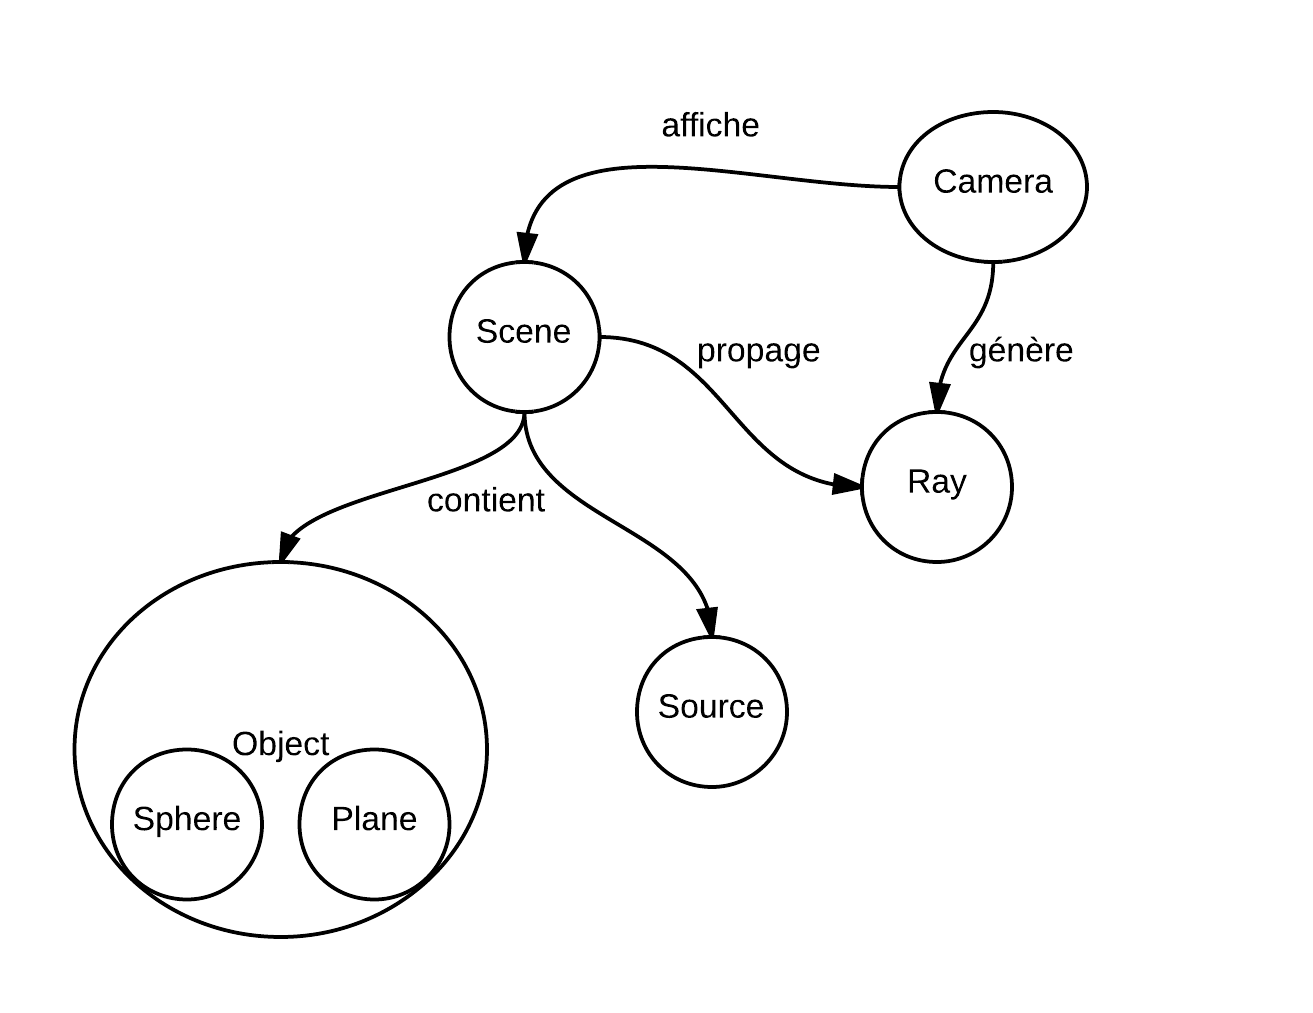
\includegraphics[height = 7cm]{schema.png}
  		\end{center}
	\end{frame}	
		
	
























\end{document}
